\section{Theorie}
\label{sec:Theorie}

\cite{sample}

\subsection{Funktionsweise}
Das Geiger-Müller-Zählrohr misst die Intensität ionisierender Strahlung. Es besteht aus einem Kathodenzylinder und einem axialen
Anodendraht.

\begin{figure}[H]
  \centering
  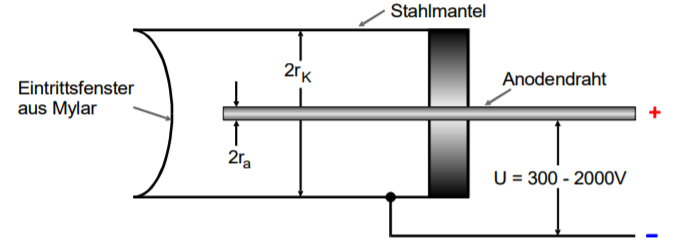
\includegraphics[height=5cm]{geigerzaehler.PNG}
  \caption{Aufbau eines Geiger-Müller-Zählrohrs \cite{sample}}
  \label{fig:Linienspektrum}
\end{figure}

 Im Innern ist ein Gasgemisch, welches durch von außen eintretende Teilchen ionisiert werden kann. Ebenfalls wird in Innern ein elektrisches
 Feld angelegt, damit die durch Ionisation entstehenden Elektronen den Draht erreichen. Ist die angelegte Spannung zu klein,
 rekombinieren die meisten Elektronen bevor sie den Draht erreichen.

 \begin{figure}[H]
   \centering
   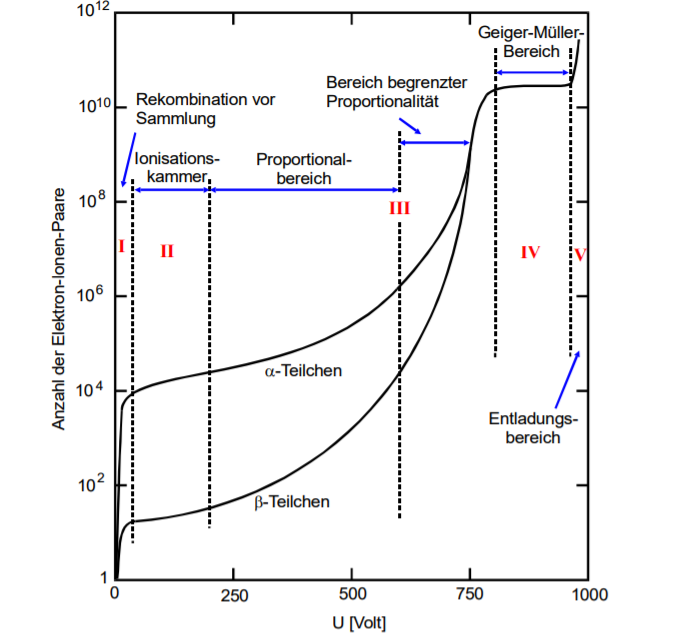
\includegraphics[height=8cm]{zonen.PNG}
   \caption{Zahl der entstehenden Elektronen in Abhängigkeit von der Spannung. \cite{sample}}
   \label{fig:Linienspektrum}
 \end{figure}

 In Abbildung 2 ist das Verhältnis zwischen Spannung und entstehenden Elektronen dargestellt. Erst ab Bereich II
erreichen so gut wie alle Elektronen den Draht bevor sie rekombiniert werden. Der entstehende Ionisationsstrom ist
proportional zur Energie und der Intensität der einfallenden Strahlung.

Bei hinreichend großer Spannung (Bereich III) haben die freigesetzten Elektronen ebenfalls genug Energie um das Argongas zu ionisieren,
wodurch die Anzahl an freigesetzten Elektronen stark ansteigt.

Das Zählrohr arbeitet jedoch hauptsächlich in Bereich IV. Bei einer dementsprechenden Spannung bleiben Entladungen nicht
auf lokalisierte Elektronenlawinen beschränkt, sondern breiten sich im ganzen Zählrohr aus. Dies liegt
an UV-Photonen die durch die primäre Elektronenlawine entstehen und weitere Elektronen freisetzen. Die
daraus folgenden elektrischen Impulse sind groß genug um sie zu messen.

\subsection{Totzeit, Erholungszeit und Nachentladung}

Die positiven Ladungsträger halten sich, wegen ihrer großen Masse, länger im Zählrohr auf. Sie bauen ein eigenes
elektrisches Feld auf, welches dem E-Feld des Geiger-Müller-Zählrohrs entgegenwirkt und somit die Elektronen abbremst.
Dadurch können diese nicht mehr ihr um liegendes Gas ionisieren, wodurch ein einfallendes Teilchen in dieser Zeit
nicht registriert werden kann. Diese Zeitspanne $T$ in der kein Teilchen registriert werden kann, wird Totzeit genannt
und folgt auf eine Entladung, da dort die positiven Ladungsträger freigesetzt werden.
Bei der Zwei-Quellen-Methode (in der Durchführung erläutert) gilt für die Totzeit:
\begin{align}
  T \approx \frac{N_1 + N_2- N_{1+2}}{2 N_1 N_2}
\end{align}

Dabei ist $N_1$ und $N_1$ die Zählrate für die zwei Strahler und $N_{1+2}$ die Zählrate,
wenn beide Strahler eingesetzt werden.

Die Erholungszeit beschreibt den Zeitraum nach der Totzeit, in dem die positive Ladungswolke zu dem Zählrohrmantel steigt und somit
das Feld des Geiger-Müller-Zählrohrs wieder stärker wird. in dieser Zeit haben die Ausgangsimpulse eine geringere Höhe.


\begin{figure}[H]
  \centering
  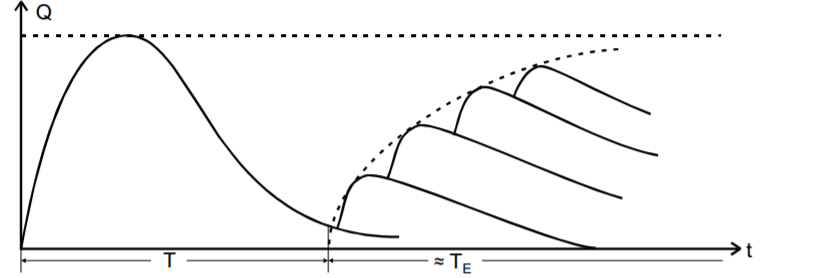
\includegraphics[height=5cm]{totzeit.PNG}
  \caption{Totzeit und Erholungszeit eines Geigerzählers. \cite{sample}}
  \label{fig:totzeit}
\end{figure}

Aus dem Zählrohrmantel können weitere Elektronen durch die auftreffenden Ionen ausgelöst werden, diese können eine weitere,
zeitlich versetzte Elektronenlawine auslösen. Dadurch wird eine einfallendes Teilchen vorgetäuscht, was zu einer
fehlerhaften Messung führt. Dieser Vorgang wird Nachentladung genannt. Um eine Nachentladung zu unterbinden, befindet
sich neben dem Argongas zusätzlich Alkoholdampf in dem Geiger-Müller-Zählrohr. Diese Alkoholdämpfe
werden von den Ladungsträgern ionisiert und treffen an deren Stelle auf den Zählrohrmantel. Dort werden nun keine
Elektronen ausgelöst, sondern lediglich die Alkoholmoleküle zum Schwingen angeregt.

\subsection{Charakteristik eines Zählrohrs}

Wird für ein  Geiger-Müller-Zählrohr die Zahl an registrierten Teilchen, bei konstanter Strahlintensität, gegen die Spannung
aufgetragen, ergibt sich die sogenannte Charakteristik.

\begin{figure}[H]
  \centering
  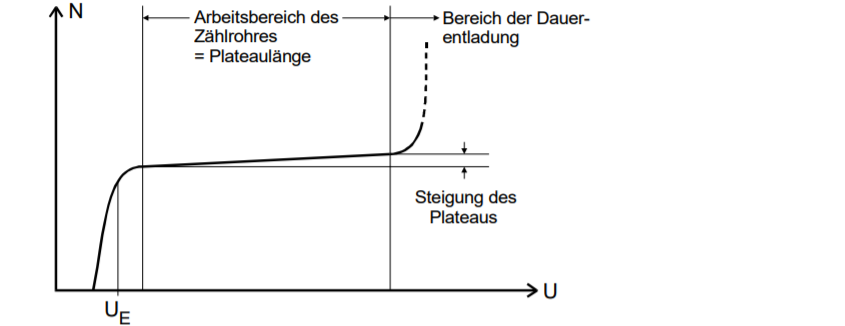
\includegraphics[height=7cm]{charakteristik.PNG}
  \caption{Charakteristik eines Zählrohrs \cite{sample}}
  \label{fig:Linienspektrum}
\end{figure}

Der Auslösebereich fängt ungefähr bei $U_E$ an. Innerhalb des darauf folgenden Plateaus sollte die
Anzahl an gemessenen Teilchen gleich bleiben. In der Realität entstehen jedoch immer wenige Elektronen durch die Nachentladung,
da diese nicht vollständig verhindert werden kann.

Bei noch größeren Spannungen löst ein einzelnes Teilchen schon eine Dauerentladung aus, was zu einer schnellen Zerstörung
des Zählrohrs führt.


\subsection{Freigesetzte Ladungsmenge pro Teilchen}

Für den mittleren Zählrohrstrom $\overline{\symup{I}}$, welcher in dem Geiger-Müller-Zählrohr gemessen werden kann gilt:
\begin{align}
  \overline{\symup{I}} = \frac{\Delta Q}{\Delta t} Z
\end{align}

Hierbei ist $\Delta Q$ die pro Zeitintervall $\Delta t$ einfallende transportierte Ladung und $Z$ die Anzahl an Teilchen die in diesem
Zeitintervall registriert werden.
